% Alten Labs Template
% Modified from the UCT Project report by Linus C. Brendel
% https://www.overleaf.com/latex/templates/uct-report-template/

%------------------------------------------------------
% DO NOT MODIFY THE FOLLOWING
\documentclass[a4paper,12pt]{article}

\usepackage[spanish]{babel}
\bibliographystyle{ieeetr}
\usepackage{url}
\usepackage{listings}
\usepackage{color} %red, green, blue, yellow, cyan, magenta, black, white
\usepackage[utf8]{inputenc}
\usepackage{amsmath}
\usepackage{graphicx}
\graphicspath{{images/}}
\usepackage{parskip}
\usepackage{fancyhdr}
\usepackage{vmargin}
\usepackage[T1]{fontenc}
\usepackage{setspace}
\usepackage{titlesec}

% Interlineado simple a 6 puntos
% \singlespacez
\setlength{\parskip}{6pt} 

\titlespacing*{\section}{0pt}{2pt}{2pt}
\titlespacing*{\subsection}{0pt}{1pt}{1pt}


%\setmarginsrb{leftmargin}{topmargin}{rightmargin}{bottommargin}%{headheight}{headsep}{footheight}{footskip}
% Margenes de 2.5 cm a ambos lados del texto
\setmarginsrb{2.43 cm}{0.9 cm}{2.43cm}{1 cm} {0.9 cm}{0.9 cm}{0.9 cm}{0.9cm}

% remove serifs ( tipografía sin remates )
% \sffamily
\renewcommand{\familydefault}{\sfdefault}
%---------------------------------------------------------------------
% If you are including code snips or putting code in your appendix, you can define
% the colors used here.  See the listings example in the appendix for including 
% source code such as MatLab or Arduino.

%---------------------------------------------------------------------
%                           COULEURS ALTEN
%---------------------------------------------------------------------

\definecolor{darkblue}{RGB}{219, 48, 122}
\definecolor{blue}{RGB}{0, 139, 210}
\definecolor{lightblue}{RGB}{126, 203, 238}
\definecolor{orange}{RGB}{255, 186, 0}



% This is your title for your report.  It should include the milestone number and what this Milestone is about.
\title{Una estrategia de Meta-Learning para flujos genéricos de AutoML.}
%This should be the team leader
\author{Loraine Monteagudo García}
% Here enter all the names that contributed to this report.  This should be all the team members.
\newcommand{\members}{Member 1}
%This will automatically put today's date
\date{ }

%Here is the role for each person listed.  It is in the same order as the author and then members.
\newcommand{\role}{loraine.monteagudo@matcom.uh.cu}
%Insert your faculty adviser here
\newcommand{\faculty}{Facultad de La Habana}
%Insert your project name here
\newcommand{\project}{Concurso Nacional de Computación 2021}
%Iinsert your team name here
\newcommand{\team}{Carreras afines a la computación}

\newcommand{\thetutors}{Dr. Suilan Estévez Velarde, \\ Lic. Daniel Alejandro Valdés Pérez}

\newcommand{\tutormails}{sesteves@matcom.uh.cu \\ daniel.valdes@matcom.uh.cu}

\newcommand{\degree}{Ciencia de la Computación, Quinto curso}

\newcommand{\dyear}{Quinto}



%------------------------------------------------------------------------
%DO NOT MODIFY ANY OF THE FOLLOWING ITEMS
%------------------------------------------------------------------------
\makeatletter
\let\thetitle\@title
\let\theauthor\@author
\let\thedate\@date
\makeatother

\pagestyle{fancy}
\fancyhf{}
\renewcommand{\footrulewidth}{1pt}
\rhead{
\includegraphics[width=1cm]{logo-uh.png}}
\setlength\headheight{33pt} 
\lhead{\thetitle}
\cfoot{\thepage}
%\rfoot{C1-Interne /C2-Restreint/C3-Secret}


\begin{document}

\begin{titlepage}
	\centering
    
\includegraphics[scale = 0.4]{logo-uh.png}\\[1.0 cm]
    \textsc{\LARGE Universidad de La Habana}\\[1.0 cm]	
	\rule{\linewidth}{0.2 mm} \\[0.4 cm]
	{ \huge \bfseries \thetitle}\\
	\rule{\linewidth}{0.2 mm} \\[1.0 cm]
    %\emph{Trabajo:}
    \project \ \\
    \emph{Modalidad:}
    \team \\
    \emph{Carrera:}
    \degree \\[1.0 cm]
	
	\begin{minipage}{0.4\textwidth}
		\begin{flushleft} \large
			\emph{Autor(es):}\\
			\theauthor \\
			\end{flushleft}
			\end{minipage}~
			\begin{minipage}{0.4\textwidth}
			\begin{flushright} \large
			\emph{} \\
			\role
		\end{flushright}
	\end{minipage}\\[1.0 cm]
	
	\begin{minipage}{0.4\textwidth}
		\begin{flushleft} \large
			\emph{Tutor(es):}\\
			\thetutors \\
			\end{flushleft}
			\end{minipage}~
			\begin{minipage}{0.4\textwidth}
			\begin{flushright} \large
			\emph{} \\
			\tutormails
		\end{flushright}
	\end{minipage}\\[1 cm]
	
	{\large Facultad de Matemática y Computación}\\[1 cm]
	
 
	\vfill
	
\end{titlepage}

%%%%%%%%%%%%%%%%%%%%%%%%%%%%%%%%%%%%%%%%%%%%%%%%%%%%%%%%%%%%%%%%%%%%%%%%%%%%%%%%%%%%%%%%

\section*{Resumen}

El campo de aprendizaje de máquinas automático (AutoML) se ha destacado como una de las principales alternativas para encontrar buenas soluciones para problemas complejos de aprendizaje automático. A pesar del reciente éxito de AutoML, todavía quedan muchos desafíos. El aprendizaje de AutoML es un proceso costoso en tiempo y puede llegar a ser ineficiente computacionalmente. Meta-Learning es descrito como el proceso de aprender de experiencias pasadas aplicando varios algoritmos de aprendizaje en diferentes tipos de datos y, por lo tanto, reduce el tiempo necesario para aprender nuevas tareas. Una de las ventajas de las técnicas de meta-learning es que pueden servir como un apoyo eficiente para el proceso de AutoML, aprendiendo de tareas previas los mejores algoritmos para resolver un determinado tipo de problema. De esta manera, es posible acelerar el proceso de AutoML, obteniendo mejores resultados en el mismo período de tiempo. El objetivo de esta tesis es diseñar una estrategia de meta-learning para dominios genéricos en el aprendizaje automático.
\setcounter{page}{0}

\subsubsection*{Palabras clave:}
Aprendizaje Automático, Meta-Learning, AutoML

\newpage

%%%%%%%%%%%%%%%%%%%%%%%%%%%%%%%%%%%%%%%%%%%%%%%%%%%%%%%%%%%%%%%%%%%%%%%%%%%%%%%%%%%%%%%%

%%%%%%%%%%%%%%%%%%%%%%%%%%%%%%%%%%%%%%%%%%%%%%%%%%%%%%%%%%%%%%%%%%%%%%%%%%%%%%%%%%%%%%%%

% \tableofcontents
% \pagebreak

%%%%%%%%%%%%%%%%%%%%%%%%%%%%%%%%%%%%%%%%%%%%%%%%%%%%%%%%%%%%%%%%%%%%%%%%%%%%%%%%%%%%%%%%

%-----------------------------------------------------------------------
% BEGIN YOUR DOCUMENT HERE
%-----------------------------------------------------------------------

%-----------------------------------------------------------------------
% INSTRUCTIONS
% This is where you will write your document.  Your table of contents will automatically get filled out based what you label as a section or subsection.  In addition, any paper, book, article or web site that you use must be cited.  This can be done using the biblist.bib file.  I have included all sections that are required and some examples.  Any images you use should go in the images folder.  This file will automatically search for images in that folder.
%===================================================================================
% Introducción
%-----------------------------------------------------------------------------------
\section{Introducción}\label{sec:intro}
%-----------------------------------------------------------------------------------
\setcounter{page}{1}
En los últimos tiempos ha habido una explosión en la investigación y aplicación del aprendizaje automático, en inglés \textit{machine learning} (ML)~\cite{hey2020machinelearning}. Sin embargo, el rendimiento de muchos métodos de aprendizaje automático es sensible a una gran variedad de decisiones~\cite{dyrmishi2019decision, radwa2019automated}, lo que constituye una barrera para nuevos usuarios~\cite{crisan2021fits}. Por ejemplo, el científico de datos debe seleccionar entre una amplia gama de posibles algoritmos, incluidas las técnicas de clasificación o regresión (como \textit{support vector machines}, redes neuronales, modelos bayesianos, árboles de decisión, etc.) y ajustar numerosos hiperparámetros del algoritmo seleccionado. Además, el rendimiento del modelo también se puede juzgar por varias métricas (por ejemplo, precisión, sensibilidad, medida F1). Incluso los expertos requieren gran cantidad de recursos y tiempo para crear modelos con buen rendimiento a causa del proceso de prueba y error que es repetido en cada aplicación para desarrollar modelos eficientes de aprendizaje automático.

Por estas razones ha emergido una nueva idea para automatizar el proceso de ML, aprendizaje de máquinas automático, denominada \textit{Automated Machine Learning} o AutoML. AutoML abarca el diseño de técnicas para automatizar y facilitar todo el proceso de implementación, experimentación y despliegue de algoritmos de aprendizaje automático. AutoML está concebido para reducir la carga de trabajo de los científicos de datos y permitir a los expertos construir automáticamente aplicaciones de ML sin mucho conocimiento en el campo. Por lo tanto, AutoML hace accesible enfoques de aprendizaje automático a los usuarios no expertos que están interesados en aplicarlos, pero no tienen los recursos para aprender sobre las tecnologías involucradas en detalle~\cite{hutter2019autmlbook}.

Sin embargo, una de las limitaciones presentes en los primeros sistemas de AutoML consiste en su inhabilidad de reusar conocimiento previo para solucionar nuevas tareas~\cite{dyrmishi2019decision}. Para cerrar esta brecha, las herramientas de AutoML comenzaron a aplicar técnicas de meta-learning, las cuales tienen el objetivo de obtener modelos para nuevas tareas usando experiencias previas. Meta-learning, o \textit{aprender a aprender}, es la ciencia de observar sistemáticamente cómo se desempeñan los diferentes enfoques de aprendizaje automático en una amplia gama de tareas de aprendizaje, y luego aprender de esta experiencia, o meta-datos, para aprender nuevas tareas mucho más rápido de lo que sería posible de otra manera. Esto no solo acelera y mejora drásticamente el diseño de algoritmos de aprendizaje automático, sino que también nos permite reemplazar algoritmos diseñados a mano con enfoques novedosos aprendidos de una manera basada en datos. Este tipo de estrategias ayudan a disminuir el costo de aplicar AutoML, al relacionar un nuevo conjunto de datos con los mejores flujos obtenidos en problemas similares previamente resueltos. 

En los recientes años se ha desarrollado un substancial interés en el campo de meta-learning y muchos sistemas de AutoML lo han integrado~\cite{fuerer2015efficient, maher2019smartml, drori2018alphad3m, yang2018oboe, zimmer2021auto, Feurer2020AutoSklearn2T}. Sin embargo, estas herramientas de meta-learning no son suficientemente flexibles para ser utilizadas en problemas prácticos que requieren la combinación de algoritmos y tecnologías de diferente naturaleza. Las técnicas actuales de meta-learning se centran principalmente en un subconjunto específico de algoritmos, a menudo adaptados a una biblioteca o conjunto de herramientas. Resolver problemas complejos, por otro lado, requiere la combinación de diferentes herramientas que podrían no estar disponibles en una misma biblioteca. Para la aplicación de meta-learning es necesario la representación de estos problemas mediante caracterizaciones informativas para los datasets y representaciones descriptivas para las soluciones obtenidas mediante diferentes herramientas. De esta forma, es posible que meta-learning sea capaz de resolver una gran cantidad de tareas.

El objetivo general de este trabajo es el diseño de una estrategia de meta-learning para métodos genéricos de AutoML, a partir de la combinación de técnicas de aprendizaje automático y optimización. La estrategia implementada tendrá el objetivo de acelerar el proceso de búsqueda de AutoML añadiendo conocimiento previo, de tal manera que se obtengan mejores resultados en el mismo período de tiempo.

 Dado un dataset, una tarea de evaluación (por ejemplo, clasificación o regresión), el algoritmo de meta-learning propuesto tiene el objetivo de producir una lista de los modelos candidatos, basada en el rendimiento esperado de estos modelos en el dataset dado. Esta lista es producida solamente con meta-conocimiento ganado del análisis de datasets relacionados y el entrenamiento de combinaciones de algoritmos en dichos datasets, sin ejecutar ninguno de los algoritmos candidatos. Teniendo este meta-conocimiento, es posible estimar el rendimiento de esos flujos y sugerirlos. Esta estimación, aunque no es exacta, mejorará el proceso de búsqueda de sistemas de aprendizaje de máquinas automático.

 El enfoque de meta-learning propuesto está compuesto por dos fases principales: la fase offline, de aprendizaje y la fase online, de recomendación. El objetivo de la fase offline es obtener los meta-datos necesarios para la solución del problema de meta-learning propuesto: la obtención de un ranking de modelos de aprendizaje para una determinada tarea. En esta fase se obtiene una caracterización de los datasets y el rendimiento y la estructura de un conjunto soluciones en dichos datasets. Por otro lado en la fase online, dada una tarea con los meta-datos ganados del análisis de las tareas similares y el entrenamiento de un conjunto de algoritmos en dichos datasets, el objetivo es producir una lista de las soluciones prometedoras para resolver la tarea inicial. Esta lista será utilizada para sugerir rápidamente algunas inicializaciones para el proceso de búsqueda de algoritmos de AutoGOAL.

%===================================================================================



%===================================================================================
% Estado del Arte
%-----------------------------------------------------------------------------------
\section{Estado del Arte}\label{sec:review}
%-----------------------------------------------------------------------------------
% El área de interés de esta investigación es la aplicación de meta-learning para la selección de modelos, en concreto, su utilización para añadir conocimiento en sistemas AutoML, por lo que varias técnicas para la solución de este problema son estudiadas.

%-----------------------------------------------------------------------------------
% 	\subsection{Meta-Learning}\label{sub:metalearning}
% %-----------------------------------------------------------------------------------
% Meta-learning es mejor entendido comúnmente como ``aprendiendo a aprender'', lo cual se refiere al proceso de mejorar un algoritmo de aprendizaje a través de múltiples episodios de aprendizaje. En contraste, el aprendizaje automático convencional mejora las predicciones del modelo sobre múltiples instancias de datos. Durante el \textit{base-learning} o aprendizaje base, un algoritmo de aprendizaje interior (o inferior/base) resuelve una tarea como clasificación de imágenes, definida por un dataset y un objetivo. Durante \emph{meta-learning}, un algoritmo externo (o superior/meta) actualiza el algoritmo interior de tal manera que el modelo que aprende mejora un objetivo externo. Los episodios de aprendizaje de la tarea base pueden ser vistos como una forma de proveer las instancias necesitadas por el algoritmo externo para aprender el algoritmo de aprendizaje base~\cite{hospedales2021metalearning}. 

% Meta-learning difiere de \textit{base-learning} en el alcance del nivel de adaptación. Mientras que el aprendizaje en un nivel base está enfocado en acumular experiencia en una tarea específica, el aprendizaje en meta-learning tiene el objetivo de acumular experiencia en el rendimiento de múltiples aplicaciones de un sistema de aprendizaje. De esta forma, muchos algoritmos convencionales tales como la búsqueda aleatoria de hiperparámetros mediante validación cruzada podrían caer en la definición de meta-learning. La característica destacada del \emph{meta-learning} contemporáneo es un meta-objetivo explícitamente definido, y una optimización de extremo a extremo del algoritmo interior con respecto a este objetivo.

% Un sistema de meta-learning está compuesto esencialmente por dos partes. Una parte tiene la tarea de adquirir meta-conocimiento de sistemas de aprendizaje automático. La otra parte tiene el objetivo de aplicar este meta-conocimiento a nuevos problemas con el objetivo de identificar un algoritmo o técnica de aprendizaje óptimo~\cite{bradzil2017metalearning}.

% Meta-learning puede ser empleada en una variedad de configuraciones, con cierto desacuerdo en la literatura sobre lo que constituye exactamente un problema de meta-learning. Meta-learning es extremadamente útil en los casos donde es requerido un modelo de aprendizaje automático y hay poca cantidad de datos, ya que el modelo contiene muchos parámetros que no pueden ser estimados precisamente con pocos datos. Algunas de las aplicaciones comunes son en la investigación robótica, donde se espera que los robots tengan un mayor nivel de autonomía en IA, en el descubrimiento de drogas para manejar los datos de altas dimensiones con un tamaño de muestra pequeño y en la traducción de lenguajes raramente usados~\cite{peng2020comprehensive}. Además, meta-learning es ampliamente empleado en el problema de selección de algoritmos, sobre esta aplicación se profundiza en la Sección \ref{sub:metalearning-automl}.

% Meta-learning constituye una solución factible para los problemas donde una definición específica de ``tarea'' y ``etiqueta'' puede ser claramente distinguida. Un sistema de meta-learning es flexible y puede ser integrado convenientemente con la mayoría de los algoritmos de aprendizaje automático para proporcionar soluciones factibles~\cite{peng2020comprehensive}. Para las tareas que son computacionalmente costosas, meta-learning presenta la opción de agregación o adaptación de los resultados anteriores para salvar recursos computacionales.
 

%-----------------------------------------------------------------------------------
% 	\subsection{AutoML}\label{sub:automl}
% %-----------------------------------------------------------------------------------

% \textit{Automated Machine Learning} (AutoML) o Aprendizaje de Máquinas Automático es el campo que se enfoca en los métodos que tienen el objetivo de automatizar diferentes etapas del proceso de aprendizaje automático. Como su nombre indica, AutoML es la intersección de dos campos: automatización y ML. Las soluciones de AutoML están recibiendo incrementalmente más atención tanto por la comunidad de ML como por los usuarios por las grandes cantidades de datos disponibles en todas partes y la falta de expertos de aprendizaje automático que puedan supervisar/asesorar el desarrollo de sistemas basados en ML~\cite{hutter2019autmlbook}.

% La comunidad de AutoML se ha centrado en resolver varias partes de un flujo de trabajo de aprendizaje automático estándar. Algunos ejemplos de estas partes o subtareas que son aplicadas en AutoML son:

% \begin{itemize}
% 	\item Preparación Automática de Datos o \textit{Automated Data Preparation}
	
% 	\item Ingeniería Automática de Características o \textit{Automated Feature Engineering}
	
% 	\item Búsqueda de Arquitecturas Neuronales o \textit{Neural Architecture Search} (NAS)
% \end{itemize}

% Sin embargo, los estudios recientes de AutoML buscan automatizar el flujo de algoritmos de aprendizaje automático entero~\cite{fuerer2015efficient, olson2019tpot, paszke2019pytorch, chen2018autostacker, swearingen2017atm}. Un flujo de algoritmos es una forma de codificar y automatizar el flujo de trabajo necesario para producir un modelo de aprendizaje automático. Los flujos de algoritmos de aprendizaje automático constan de varios pasos secuenciales que realizan desde la extracción de datos y el preprocesamiento hasta el entrenamiento y la implementación del modelo~\cite{web-mlpipe}.

% Dos problemas importantes en AutoML son que ningún algoritmo de ML obtiene los mejores resultados en todos los datasets, también conocido como \textit{No Free Lunch Problem} \cite{wolpert1995no}, y que algunos métodos de aprendizaje automático dependen crucialmente de la optimización de hiperparámetros. Para la resolución de estos problemas AutoML se apoya de dos áreas o subtareas que constituyen su base: la selección de modelos (\textit{Model Selection}, MS)~\cite{thornton2013auto} y la optimización de hiperparámetros (\textit{Hyperparameter Optimization}, HPO)~\cite{fuerer2019hyperparameter}. La combinación de estas áreas se refiere al problema de AutoML como un problema de selección combinada de modelos y optimización de hiperparámetros (\textit{Combined Algorithm Selection and Hyperparameter Optimization}, CASH)~\cite{thornton2013auto}.

% Con el objetivo de abordar el problema de CASH el proceso de AutoML consta de tres componentes que definen el proceso de optimización:

% \begin{description}
% 	\item[Espacio de Búsqueda:] precisa los algoritmos y todos los rangos válidos para sus hiperparámetros que son posibles soluciones para un problema de AutoML concreto. Además, se pueden optimizar combinaciones complejas de algoritmos, en cuyo caso las restricciones de compatibilidad entre algoritmos también son modeladas.
% 	\item[Estrategia de Búsqueda:] detalla como se explora el espacio de búsqueda, que puede ser de tamaño exponencial o ilimitado. Se ve afectado por el clásico problema de Exploración vs. Explotación, ya que se quieren encontrar soluciones de alto rendimiento rápidamente, pero se debe evitar converger prematuramente a regiones subóptimas de búsqueda.
% 	\item[Estrategias de Estimación de Rendimiento:] son mecanismos para estimar la capacidad predictiva de las soluciones encontradas por los sistemas de AutoML.
% \end{description}

% La estrategia de búsqueda es el proceso que sustituye la búsqueda de los hiperparámetros realizada por los humanos. Este procedimiento requiere tiempo y recursos considerables debido a los métodos de prueba y error que son necesitados para buscar el mejor modelo y su configuración de hiperparámetros. Por lo tanto, muchos métodos de optimización han surgido con el objetivo de acelerar esta búsqueda para liberar a los humanos de este tedioso proceso y para explorar el espacio de búsqueda definido de forma automática. Este proceso de optimización es el que pretende imitar el rol de los expertos y es el núcleo fundamental para resolver el problema de CASH. Algunos ejemplos de las estrategias de búsquedas más usadas son:

% \begin{description}
% 	\item[Grid Search y Random Search:] \textit{Grid Search} (GS) es el proceso de discretizar cada hiperparámetro y evaluar exhaustivamente cada combinación de valores. Por otro lado, \textit{Random Search} (RS) o búsqueda aleatoria configura una cuadrícula de valores de hiperparámetros y selecciona combinaciones aleatorias para entrenar el modelo. Esto permite controlar explícitamente el número de combinaciones de parámetros que se intentan. Algunos sistemas de AutoML que han implementado versiones de estas estrategias son: Hyperopt~\cite{bergstra2013hyperopt}, Rafiki~\cite{wang2018rafiki} y FLAML~\cite{wang2021flaml}.
%  	\item[Optimización Bayesiana:] BO es un algoritmo iterativo, cuya idea clave es modelar la asignación entre un conjunto de hiperparámetros $\lambda$ y da como resultado una estimación de su rendimiento $\hat{c}(\lambda)$ basado en valores de rendimiento observados encontrados en un archivo $A$ mediante regresión no lineal. Este modelo aproximado se denomina modelo sustituto, o modelo probabilístico, para el cual es normalmente utilizado un proceso gausiano o un bosque aleatorio. Esta estrategia de búsqueda ha sido utilizada por los siguientes sistenmas: Auto-WEKA~\cite{thornton2013auto}, Hyperopt~\cite{bergstra2013hyperopt}, Auto-Sklearn~\cite{fuerer2015efficient}, Auto-Net~\cite{mendoza2016towards} y Auto-Keras~\cite{jin2019auto}
%   	\item[Algoritmos Evolutivos:] Un algoritmo evolutivo (EA) es un subconjunto de la computación evolutiva, un algoritmo genérico de optimización metaheurística basado en la población. En un algoritmo evolutivo, una \textit{población} de soluciones candidatas (llamadas individuos, criaturas o fenotipos) en un problema de optimización evoluciona hacia mejores soluciones. Cada solución candidata tiene un conjunto de propiedades (sus cromosomas o genotipo) que se pueden mutar y alterar. En la terminología de la optimización de hiperparámetros un \textit{individuo} es una configuración de hiperparámetros única, la \textit{población} es un conjunto de configuraciones de hiperparámetros actualmente mantenido y la \textit{aptitud} de un individuo es su error de generalización. La mutación es el cambio (aleatorio) de uno o unos pocos valores de hiperparámetros en una configuración. El cruce crea una nueva configuración de hiperparámetros mezclando aleatoriamente los valores de otras dos configuraciones. Ejemplos del uso de algoritmos evolutivos el los sistemas de AutoML son: Autostacker~\cite{chen2018autostacker}, TPOT~\cite{olson2019tpot}, RECIPE~\cite{de2017recipe}, $Auto-MEKA_{GPP}$~\cite{de2018automated} y AutoGOAL~\cite{autogoal}.
%    \item[Aprendizaje por refuerzo:] El aprendizaje por refuerzo (RL), como estrategia de búsqueda, consiste en entrenar un agente que realiza modificaciones sobre una solución con el objetivo de maximizar una recompensa que depende del rendimiento de dicha solución. Es un marco de optimización muy general y sólido, que puede resolver problemas con retroalimentación retardada. A diferencia de los métodos anteriores, las retroalimentaciones (es decir, la recompensa y el estado) no necesitan ser devueltos inmediatamente una vez que se toma una acción. Se pueden devolver después de realizar una secuencia de acciones. Un ejemplo del uso de esta estrategia se encuentra en Alpha3DM~\cite{drori2018alphad3m}
%    \item[Monte Carlo Tree Search (MCTS):] Monte Carlo Tree Search (MCTS) es un algoritmo de búsqueda heurística para algunos tipos de procesos de decisión. El enfoque de MCTS es en el análisis de los movimientos más prometedores, expandiendo el árbol de búsqueda basado en un muestreo aleatorio del espacio de búsqueda. Cada ciclo de evaluación consiste en construir una solución completa, que se traduce en descender por una rama del árbol del espacio de búsqueda. En un algoritmo de Monte Carlo es necesario definir cómo se escoge el siguiente nodo a evaluar, lo que conlleva un balance entre exploración y explotación. A medida que se explora el espacio de búsqueda, se descubre qué decisiones en niveles superiores tienen un mejor rendimiento y se sesga la búsqueda hacia esas regiones del espacio. Ejemplos de la implementación de esta estrategia se encuentra en: MOSAIC~\cite{rakotoarison2019automated} 
% \end{description}

%-----------------------------------------------------------------------------------
	% \subsection{Meta-Learning para AutoML}\label{sub:metalearning-automl}
%-----------------------------------------------------------------------------------

La principal área de investigación de meta-learning estudiada en este trabajo es la selección de algoritmos, la cual ha recibido una considerable cantidad de investigación. En el caso especial de meta-learning, el aspecto de interés es la relación entre las características de los datos y el rendimiento del algoritmo, con el objetivo final de predecir un algoritmo o un conjunto de algoritmos adecuado para un problema específico. Como motivación está el hecho de que es inviable examinar todas las posibles alternativas de algoritmos en un procedimiento de prueba y error. La aplicación de meta-learning en este campo puede, por lo tanto, ser útil tanto para proveer una recomendación para un usuario final como de paso preliminar para recomendar algoritmos a soluciones más costosas computacionalmente, como los algoritmos de optimización usados en herramientas de AutoML. 


El desafío en meta-learning para la selección de modelos es aprender de experiencias pasadas de una forma sistemática e impulsada por los datos. Primero, es necesario extraer los meta-datos que describen las tareas de aprendizaje anteriores y los modelos previamente aprendidos. Estos meta-datos comprenden las configuraciones exactas de los algoritmos empleados para entrenar los modelos, incluyendo:

\begin{itemize}
	\item Las configuraciones de los hiperparámetros, composiciones de los flujos de algoritmos y/o arquitecturas de redes neuronales.
	\item Las evaluaciones del modelo resultante, tales como la precisión y el tiempo de entrenamiento.
%	\item Los parámetros del modelo aprendidos, tales como los pesos entrenados de una red neuronal.
	\item Propiedades medibles de la tarea en sí, que son extraídas de los datasets, también conocidas como meta-características.
\end{itemize}

Luego es necesario aprender de estos meta-datos previos, para extraer y transferir conocimiento de la búsqueda de los modelos óptimos para nuevas tareas. El resto de esta sección presenta una visión general de diferentes enfoques de meta-learning para hacer esto efectivamente. Además, se muestran ejemplos de cómo estos enfoques han sido utilizados como paso preliminar en varias herramientas de AutoML.

En esta sección las técnicas de meta-learning son separadas en grupos de acuerdo al tipo de meta-datos que ellas aprovechan \cite{vanschoren2018metalearning}. Primero, se discute cómo caracterizar las tareas para expresar más explícitamente la similitud entre ellas y cómo construir meta-modelos para aprender las relaciones entre las características de los datos y el rendimiento de las distintas evaluaciones de los modelos (Sección \ref{subsec:mtl_automl_proprerties}), y luego se describe como se aprende solamente de evaluaciones de los modelos (Sección \ref{subsec:mtl_automl_evaluations}).

\subsection{Aprendiendo de las propiedades de las tareas}\label{subsec:mtl_automl_proprerties}
La principal característica de esta técnica es el uso de meta-características para medir la similitud de las tareas. Así, por ejemplo, podemos usar la distancia euclidiana entre $m(t_{new})$ y $m(t_j), \forall t_j \in T$ para transferir información de las tareas más similares a la nueva tarea $t_{new}$.

Con esta técnica de meta-learning se puede entrenar un meta-modelo (o \textit{meta-learner}) $L$ que predice el rendimiento de las configuraciones recomendadas $\Theta^*_{new}$ en una nueva tarea $t_{new}$. El meta-modelo es entrenado con los meta-datos $P\cup M$, donde $P$ y $M$ son usualmente calculados de antemano, o extraídos de repositorios de meta-datos.

Cómo extraer información adecuada para caracterizar tareas específicas es una de las preguntas fundamentales en meta-learning. Investigadores han intentado contestar esta pregunta observando las características de los datasets que afectan el rendimiento de los algoritmos~\cite{Rivolli2018TowardsRE}. Estas caracterizaciones son denominadas meta-características y usualmente se encuentran divididos en cinco grupos. Estos grupos son subconjuntos de medidas de caracterización \cite{bradzil2009metalearning} que comparten similitudes entre ellas:

\begin{description}
	\item[Simple:] representan información básica sobre el dataset. Hasta un determinado punto son concebidas para medir la complejidad del problema subyacente. Algunas de las caracterizaciones incluidas en este grupo son: el número de instancias, el número de atributos, la dimensionalidad del dataset, la proporción de valores faltantes, etc. También son llamadas medidas \textit{generales}.
	
	\item[Estadísticas:] son características que capturan las propiedades estadísticas de los datos. Estas métricas capturan los indicadores de distribución de datos, tales como la media, la desviación estándar, la correlación y curtosis.
	
	\item[Teóricas de la información:] son características del campo de teoría de la información. Estas medidas están basadas en la entropía, la cual captura la cantidad de información en los datos y su complejidad.
	
	\item[Basados en modelos:] son características extraídas de un modelo inducido de los datos de entrenamiento. Las características en este grupo están caracterizadas por la extracción de información de un modelo de aprendizaje de predicción, generalmente, un árbol de decisión.
	
	\item[\textit{Landmarking}:] son características que usan el rendimiento de algoritmos de aprendizaje simples y rápidos para caracterizar los datasets. Los algoritmos deben tener diferentes sesgos y capturar información importante con un costo computacional bajo.
\end{description}

Construyendo un meta-modelo o \textit{meta-learner} $L$ podemos aprender relaciones complejas entre las meta-características de una tarea y la utilidad de una configuración específica. Dadas las meta-características $M$ de una nueva tarea $t_{new}$ este meta-modelo $L$ tiene el objetivo de recomendar la configuración más útil $\Theta_{new}^*$ para esta tarea. Existe un gran grupo de trabajos previos construyendo modelos para la selección de algoritmos y recomendación de hiperparámetros. En esta sección se usan ejemplos de varios meta-modelos de acuerdo al tipo de tarea que resuelven: pueden ser usados para rankear un conjunto determinado de configuraciones o para predecir el rendimiento de una nueva tarea.

Los meta-modelos pueden ser usados para generar un ranking de las $K$ mejores configuraciones dado un conjunto de meta-características $M$ y una nueva tarea $t_{new}$. Se obtiene así un conjunto prometedor de modelos con sus hiperparámetros para esta nueva tarea.
 
Uno de los enfoques más populares es construir un meta-modelo de \textit{K-Nearest Neighbor} (kNN) para predecir las tareas que son similares, y luego rankear las mejores configuraciones en estas tareas similares~\cite{santos2004selection, bradzil2003ranking}. 
%En uno de los enfoques seguidos se utiliza una evaluación multicriterio que toma en cuenta la precisión obtenida y el tiempo de entrenamiento de una configuración: \textit{Adjusted Ratio of Ratios} (ARR) o el Radio Ajustado de Radios para formar los rankings. Existen muchas medidas para la evaluación de un ranking determinado, el más utilizado es el coeficiente de correlación de Spearman~\cite{santos2004selection}, el cual mide la distancia del ranking recomendado al ranking ideal. 
El ranking ideal corresponde al ordenamiento correcto de los modelos candidatos para una tarea determinada.

Muchos sistemas de AutoML han seguido el enfoque de vecinos cercanos (\textit{nearest neighbor}) para predecir las tareas similares, debido a la simplicidad de esta técnica. Auto-sklearn \cite{fuerer2015efficient} fue la primera herramienta de AutoML en seguir este enfoque. Es implementado sobre \texttt{scikit-learn}~\cite{scikit-learn}, una biblioteca popular de aprendizaje automático en Python. 
%Usa 15 clasificadores, 14 métodos de preprocesamiento de características  y 4 métodos de preprocesamiento de datos. 
Este sistema mejora los métodos existentes de AutoML tomando en cuenta automáticamente la experiencia pasada en datasets similares y construyendo \textit{ensembles} de los modelos evaluados durante la optimización. Auto-sklearn introdujo la idea de meta-learning en la inicialización de la selección de modelos y el ajuste de hiperparámetros~\cite{vanschoren2018metalearning}.

SmartML~\cite{maher2019smartml} está equipado con una base de conocimiento constantemente actualizada que guarda información sobre las meta-características de todos los datasets procesados con su rendimiento asociado de los diferentes clasificadores y sus parámetros ajustados. Para cada dataset nuevo SmartML automáticamente extrae sus meta-características y busca en su base de conocimiento el algoritmo que mejor rendimiento tenga para empezar su proceso de optimización. Una vez elegido el algoritmo, usa optimización bayesiana basada en SMAC para la optimización de hiperparámetros. Sigue el mismo procedimiento basado en meta-características de Auto-sklearn para determinar datasets similares, utilizando el enfoque de vecinos cercanos, el cual está seguido por un mecanismo ponderado entre dos factores diferentes para elegir los algoritmos de los datasets similares más prometedores: la distancia euclidiana entre las meta-características del dataset y las meta-características de todos los datasets guardados en la base de conocimiento y el rendimiento de los mejores algoritmos en datasets similares.

% MOSAIC (\textbf{MO}nte-Carlo tree \textbf{S}earch for \textbf{A}lgor\textbf{I}thm \textbf{C}onfiguration) \cite{rakotoarison2019automated} es un enfoque de AutoML basado en Monte-Carlo Tree Search (MCTS), que fue presentado para manejar las estructuras híbridas de AutoML y el problema costoso de optimización de caja negra paramétrico. La novedad de MOSAIC es que aborda el problema de optimización estructural y paramétrico usando 2 estrategias asociadas: MCTS es utilizada para abordar la optimización de la estructura \textbf{a} y la optimización bayesiana es usada para abordar la optimización paramétrica de $\omega(a)$, donde el acoplamiento es asegurado mediante los modelos sustitutos.

ATOMIC (\textit{Automated Imbalanced Classification})~\cite{atomic} es un enfoque de AutoML para desarrollar soluciones de ML para abordar tareas de Aprendizaje de Dominio Desbalanceado o \textit{Imbalanced Domain Learning} (IDL) basado en meta-learning. Proporcionan un ranking de soluciones más probables de asegurar una aproximación óptima a un nuevo dominio, reduciendo drásticamente la complejidad computacional asociada a esta tarea. Esto lo llevan a cabo anticipando la pérdida de un gran conjunto de soluciones predictivas en una nueva tarea de aprendizaje desbalanceado. A diferencia de los ejemplos anteriores para la predicción de los rankings no usan el enfoque de vecinos cercanos, sino que usan como meta-modelo el algoritmo de aprendizaje XGBoost~\cite{xgboost} para generar un ranking de los algoritmos más prometedores. 

\subsection{Aprendiendo de las evaluaciones de modelos}\label{subsec:mtl_automl_evaluations}

Otro grupo de técnicas de meta-learning están basadas en aprender de evaluaciones de los modelos. En este contexto, el problema se define como, dado un conjunto de configuraciones de algoritmos de aprendizaje, tareas anteriores, evaluaciones de las tareas anteriores en dichas configuraciones y un conjunto de evaluaciones conocidas en una tarea nueva, recomendar configuraciones teninedo en cuenta los rendimientos de las configuraciones anteriores y el conjunto de evaluacions de la nueva tarea.

Estas técnicas son usadas generalmente para recomendar configuraciones y espacios de búsqueda útiles, así como transferir conocimiento de tareas empíricamente similares. Algunas de estas técnicas son explicadas a continuación. 

Supongamos que no tenemos acceso a ninguna evaluación de la nueva tarea. Aun así se puede aprender una función que dé como resultado un conjunto de configuraciones recomendadas independientes de la nueva tarea. Estas configuraciones pueden ser evaluados en la nueva tarea para seleccionar el mejor, o para inicializar otros enfoques de optimización.

Los sistemas de AutoML han incorporado esta técnica mediante el uso de portafolios, que es comúnmente creado discretizando el conjunto de algoritmos e hiperparámetros en un conjunto de configuraciones candidatas, evaluados en un gran número de tareas anteriores.

Auto-Pytorch \cite{zimmer2021auto} es un ejemplo de estos sistemas que usan portafolios para crear un conjunto inicial de flujos de algoritmos para la subsecuente optimización. Auto-Pytorch optimiza la arquitectura de red y los hiperparámetros de entrenamiento para permitir aprendizaje profundo completamente automatizado (\textit{Automated Deep Learning}, AutoDL). 
%Combina optimización \textit{multifidelity} con construcción de portafolio de un conjunto inicial, \textit{ensembling} de redes neuronales profundas (DNNs) y baselines comunes para datos tabulares.
 Auto-Pytorch simplemente empieza la primera iteración con un conjunto de configuraciones complementarias que cubren bien un conjunto de datasets de meta-entrenamiento, después de esto ejecuta un algoritmo de optimización para la búsqueda de los mejores hiperparámetros. Para esto se construye inicialmente un portafolio inicial. Para construir el portafolio offline, se realiza una ejecución de su algoritmo de optimización en cada uno de los datasets de meta-entrenamiento, dando lugar a un conjunto de candidatos. Las configuraciones de las ejecuciones individuales son entonces evaluadas en todos los datasets, resultando en una meta-matriz de rendimiento. Para cada uno de los candidatos, configuraciones son añadidas iterativamente y de forma \textit{greedy}.
 % para minimizar su \textit{relative regret} promedio sobre todos los meta datasets. En la primera iteración la mejor configuración en promedio para todos los datasets es añadida al portafolio. En todas las iteraciones subsecuentes, son añadidas configuraciones que tienden a ser más especializadas a subconjuntos de los datasets, para los cuales son posibles mejoras. 
 Las configuraciones son añadidas de esta manera hasta que un tamaño predefinido del portafolio es alcanzado. Limitando el tamaño del portafolio se balancea entre empezar con configuraciones prometedoras y la sobrecarga inducida por el primer portafolio ejecutado. Este enfoque asume (como todos los enfoques de meta-learning) que tenemos acceso a un conjunto razonable de datasets de meta-entrenamiento que son representativos de los datases de meta-prueba.

Auto-sklearn 2.0 \cite{Feurer2020AutoSklearn2T} es una extensión de Auto-sklearn~\cite{fuerer2015efficient} que presenta una técnica de meta-learning más simple y perfecciona su manera de manejar algoritmos iterativos. Debido a varios problemas encontrados en el uso de meta-características en el algoritmo de meta-learning de Auto-sklearn, proponen un nuevo enfoque libre de meta-características, haciendo uso de un portafolio, un conjunto de configuraciones complementarias que cubren tantos datasets diversos como sea posible y minimiza el riesgo de fallo cuando se enfrenta en una nueva tarea. Para ello hacen una matriz de rendimiento, guardando el rendimiento de un conjunto de algoritmos de ML en varios datasets. Luego para seleccionar algoritmos del portafolio basado en un nuevo dataset utilizan un algoritmo \textit{greedy}. Mientras el enfoque anterior de meta-learning seguido por Auto-sklearn (\textit{k-nearest neighbors}) tiene el objetivo de usar solo configuraciones que actúan bien, un portafolio es construido de tal manera que al menos hay una configuración que funciona bien, la cual además proporciona una forma diferente de diseño inicial para su algoritmo de optimización.

Las evaluaciones previas también pueden ser usadas para aprender mejores \textit{espacios de configuración}. Incluso siendo independientes de la nueva tarea, esto puede radicalmente acelerar la búsqueda para modelos óptimos, ya que solo las regiones más relevantes de los espacios de configuración son explorados. Esto es crítico cuando los recursos computacionales están limitados. 

Uno de los sistemas de AutoML que ha usado técnicas de meta-learning para aprender mejores espacios de configuración es ATM (\textit{Auto-Tuned Models}) \cite{mendoza2016towards}. ATM es un sistema de aprendizaje automático multi-método, multi-parámetro y auto optimizado para la automatización de selección de modelos y el ajuste de hiperparámetros. Su principal contribución fue la presentación de un nuevo método para organizar el espacio de búsqueda jerárquica de los métodos de aprendizaje automático. 
%Definieron un \textit{conditional parameter tree} y la hiperpartición y demostraron cómo estas abstracciones pueden ser usadas para recorrer espacios de hiperpárametros complejos.
 Emplean técnicas automáticas de meta-learning que iterativamente seleccionan entre estos espacios jerárquicos y ajustan los hiperparámetros.

Existen varias maneras de dar recomendaciones de una tarea específica, pero generalmente se necesita información sobre qué tan similar es la nueva tarea  $t_{new}$ es a las tareas anteriores $t_j \in T$. Una manera de hacer esto es evaluando un número de configuraciones recomendadas en la nueva tarea. Si luego se observa que las evaluaciones de esta tarea son similares a las observaciones en las tareas anteriores para un dataset específico, entonces basándose en evidencia empírica $t_j$ y $t_{new}$ pueden ser consideradas similares. Este conocimiento puede ser incluido para entrenar un meta-modelo que predice un conjunto de configuraciones recomendadas para $t_{new}$. Además, cada configuración seleccionada puede ser evaluada y luego incluida en la base de meta-conocimiento, repitiendo el ciclo y coleccionando más evidencia empírica para aprender cuáles tareas son similares entre sí.

El uso del rendimiento de varios algoritmos en determinados datasets ha servido para medir la similitud de las tareas en varios sistemas de AutoML. Uno de los ejemplos de esto es OBOE \cite{yang2018oboe}, que forma una matriz de errores con validación cruzada de un gran número de algoritmos de aprendizaje supervisado (algoritmos juntos con sus hiperparámetros) en un gran número de datasets. Cada fila  en la matriz representa un dataset, cada columna representa un algoritmo de ML y cada celda representa el rendimiento de un modelo particular de aprendizaje automático con sus hiperparámetros en un dataset específico. Para encontrar los mejores modelos para un dataset nuevo, OBOE ejecuta un conjunto de algoritmos rápidos, pero informativos en el nuevo dataset y usa sus errores de validación cruzada para inferir el vector de características para el nuevo dataset. 
%Para encontrar el mejor algoritmo de aprendizaje automático para un nuevo dataset, 
OBOE ejecuta un conjunto particular de modelos correspondientes a un subconjunto de columnas en la matriz de error, los cuales son estimados para ejecutar eficientemente en el nuevo dataset. El sistema tiene en cuenta 2 problemas importantes: (1) \textbf{Inicializaciones con restricciones de tiempo}: cómo elegir un modelo prometedor inicial bajo restricciones de tiempo y (2) \textbf{Active learning}: cómo mejorar la predicción inicial dando más recursos computacionales. La predicción del tiempo de ejecución de un algoritmo depende solo del número de ejemplos y las características en el dataset. El subproblema de \textit{active learning} tiene como objetivo ganar la mayor cantidad de información para guiar el proceso de selección de modelos.

PMF \cite{fusi2018advances} soluciona la tarea de la selección automática de una secuencia de algoritmos de ML de aprendizaje automático usando ideas de filtrado colaborativo y optimización bayesiana. PMF considera que dos dataset son similares si tienen evaluaciones similares en un pequeño conjunto de flujos de algoritmos y, por lo tanto, es más probable que estos datasets tengan similares evaluaciones en el resto de los flujos. En particular, PMF entrena cada flujo de aprendizaje automático en una muestra de cada dataset y entonces evalúa dicho flujo. Esto resulta en una matriz que resume el rendimiento de cada flujo de aprendizaje automático de cada dataset. El problema de predecir el rendimiento de un flujo particular en un nuevo dataset es relacionado con un problema de factorización de matrices.

%-----------------------------------------------------------------------------------
	\section{Propuesta}\label{sub:listings}
%-----------------------------------------------------------------------------------
En esta sección se presenta un método para la selección de flujos de algoritmos usando técnicas de meta-learning. Un flujo puede ser visto como un caso especial de algoritmo que aplica cada algoritmo de forma secuencial a la salida del anterior en la sucesión. Por lo tanto, como un flujo está compuesto de varios algoritmos, la búsqueda de estos y de sus hiperparámetros resulta más compleja. 

% La herramienta de meta-learning prupuesta tiene el objetivo de abarcar una gran variedad de problemas mediante la selección de meta-características capaces de representarlas. Además, explorando la interacción entre las características de los datasets y la estructura de los flujos, el método propuesto debe identificar flujos con un buen rendimiento sin realizar un análisis computacionalmente costoso. Como sistema de AutoML complementario se eligió AutoGOAL, que destaca por la gran cantidad de técnicas y herramientas que utiliza, permitiéndole resolver una amplia gama de tareas. AutoGOAL es utilizado para la generación de flujos de algoritmos para crear la base de conocimiento, por lo que, debido a la variedad de herramientas de ML que AutoGOAL utiliza, se presenta gran diversidad en los flujos guardados.

El enfoque desarrollado se propone como un paso preliminar para otras soluciones más costosas computacionalmente, como por ejemplo, para la inicialización de sistemas de AutoML. En esta investigación AutoGOAL también es utilizado como herramienta complementaria en el proceso de búsqueda de flujos. Por lo tanto, se describe como se realiza la incorporación de conocimiento experto a la estrategia de búsqueda usada por AutoGOAL: Evolución Probabilística Gramatical (\textit{Probabilistic Grammatical Evolution})~\cite{pge2015}, que no había sido utilizada anteriormente con meta-learning.

El enfoque de meta-learning propuesto está compuesto por dos fases:
\begin{itemize}
	\item La fase offline, que es de aprendizaje, es donde ocurre la adquisición de meta-conocimiento. El objetivo de esta parte es obtener los meta-datos necesarios para la solución del problema de meta-learning propuesto: la obtención de un ranking de flujos de algoritmos de aprendizaje para una determinada tarea. En esta fase se obtiene una caracterización de los datasets y el rendimiento de un conjunto flujos de algoritmos en dichos datasets.
	\item La fase online, que es de recomendación, es donde se aplica el meta-conocimiento adquirido en la fase anterior. En esta fase, dada una tarea con los meta-datos ganados del análisis de las tareas similares y el entrenamiento de flujos de algoritmos en dichos datasets, el objetivo es producir una lista de los flujos prometedores para resolver la tarea inicial.
\end{itemize}

La Figura~\ref{fig:system} muestra el flujo de trabajo de la estrategia de meta-learning implementada. En la fase offline (Figura~\ref{fig:system} derecha) se obtiene una caracterización de los datasets y la estructura y rendimiento de un conjunto flujos de algoritmos en dichos datasets, esta información es utilizada para entrenar el meta-modelo. En la fase online (Figura~\ref{fig:system} izquierda), dado un nuevo dataset, se extraen sus meta-características y de acuerdo a estas y a una métrica de distancia se seleccionan los datasets similares. De estos datasets se obtienen los flujos de algoritmos guardados en la base de conocimiento, y con estos y el meta-modelo se genera un ranking final.

%-----------------------------------------------------------------------------------
	\subsection{Adquisición de Meta-Conocimiento}
%-----------------------------------------------------------------------------------
  	% Las referencias deben estar agrupadas en una sección al final del artículo,
  	% y las citas numeradas correctamente, por ejemplo \cite{knuth} o \cite{goedel}.
  	% Incluya toda la información importante de cada referencia, incluídos autor,
  	% título, y notas de la edición. En caso de citar sitios web, además
  	% de la URL, incluya la fecha en que fue consultado, como en \cite{wiki}. Numere 
  	% las referencias según el orden en que se les cita.

	La adquisición de meta-conocimiento se realiza mediante la extracción de caracterizaciones de un conjunto de datasets, es decir, meta-características, y de información referente a un conjunto de algoritmos que deben ser probados en estos datasets. Entre los datos de los algoritmos extraídos se guarda información respecto a los hiperparámetros utilizados y al rendimiento alcanzado en cada una de las tareas para cada uno de los conjuntos de algoritmos usados.

	Las meta-características utilizadas para describir los datasets fuerons:
	\begin{itemize}
		\item \textbf{Simples}: Supervisado, Tamaño de la muestra, Número de clases, Dimensionalidad de la entrada, Dimensionalidad de la salida, Dimensionalidad del dataset, Cantidad de características categóricas, Características categóricas, Cantidad de características numéricas, Características numéricas, Cantidad de valores faltantes.
		\item \textbf{Estadísticos}: Desviación estándar, Coeficiente de variación, Covarianza media, Coeficiente de correlación lineal, \textit{Skewness} (Oblicuidad), Curtosis, PCA (\textit{Principal Component Analysis}, Análisis de los Componentes Principales).
		\item \textbf{Teóricos de la Información}: Entropía normalizada de una clase, Entropía normalizada de un atributo, Entropía conjunta, Información mutua de clase y atributo, Número equivalente de atributos, Relación de la señal de ruido.
		\item \textbf{Específicos de AutoGOAL}: Tipo semántico de la entrada y de la salida.
	\end{itemize}

	Además de las meta-características, se extrajo información relacionada con las soluciones de las tareas, que fueron utilizadas como características para el meta-modelo. En la fase de adquisición de conocimiento, las soluciones de las tareas deben ser generadas. El enfoque de meta-learning implementado no intenta simplemente determinar un buen algoritmo con sus hiperparámetros como solución, sino un flujo de algoritmos, lo que complica la generación de estos. 
	
	Para la generación de los flujos de algoritmos se utilizó AutoGOAL. En cada uno de los datasets se ejecutó AutoGOAL y se guardaron las arquitecturas generadas junto con su rendimiento. El formato en el que se guardaron fue dependiente de la estructura en la que AutoGOAL procesa los flujos. Los algoritmos se ponen primero secuencialmente, luego existe una palabra clave \texttt{End} para representar el final de estos. Después, se ponen los hiperparámetros de los algoritmos de la forma  `\texttt{\{algoritmo\}\_\{hiperparámetro\}}' para identificarlos.

%===================================================================================
	\subsection{Aplicación de Meta-Conocimiento}
%===================================================================================

En un sistema de meta-learning la aplicación de meta-conocimiento puede ser utilizado para ayudar a seleccionar un conjunto de algoritmos de aprendizaje de máquinas que obtengan un buen rendimiento en una tarea determinada. Una vez obtenidos los meta-datos necesarios, el objetivo de esta fase es la obtención de una lista de flujos de algoritmos prometedores para un dataset determinado. Esto se realiza analizando los datasets similares a un nuevo dataset y recomendando los flujos que tuvieron un buen rendimiento en estos conjuntos de datos seleccionados. 

La selección de algoritmos fue realizada mediante un enfoque de ranking, en el que para un nuevo dataset se seleccionan los \texttt{k} mejores flujos de algoritmos. Para esto se implementaron varias estrategias, que son descritas a continuación.

	\subsubsection{Estrategia de Vecinos Cercanos}\label{subsub:nn}
	
	La primera estrategia, de \textit{Nearest Neighbors} o Vecinos Más Cercanos, consiste en extraer los flujos candidatos para un dataset determinado en dependencia de las características de los \texttt{n} datasets más similares a él. Se extraen los \texttt{m} flujos de algoritmos que hayan tenido mejor rendimiento en cada uno de los \texttt{n} datasets, y estos flujos son combinados para formar un nuevo ranking para el nuevo dataset. Este enfoque puede ser dividido en dos pasos: la búsqueda de los vecinos cercanos y la generación de un ranking.

	Una de las desventajas de este enfoque es la necesidad de especificar y determinar los mejores valores para la cantidad de datasets similares seleccionados \texttt{n} y la cantidad de flujos de algoritmos seleccionados \texttt{m}. Por lo cual, se desarrolló otro enfoque.

	El otro método para la generación de rankings consiste en un mecanismo ponderado entre dos factores: la distancia entre el nuevo dataset y los datasets del conjunto de entrenamiento, y el valor del resultado de rendimiento de los flujos de algoritmos en los dataset similares. La estrategia seguida para la combinación de estos fue una de las más directas: la división entre el resultado de rendimiento de un flujo de algoritmos en un dataset similar y el valor de distancia entre los dataset. De esta forma, los datasets que tengan menor distancia entre sí y los flujos que tengan un mejor rendimiento obtendrán un mayor resultado. Los resultados de esta división son los utilizados para generar el ranking de los flujos candidatos para la nueva tarea.

	\subsubsection{Estrategia utilizando un Meta-Modelo}\label{subsub:ranker}

	La segunda estrategia utiliza un meta-modelo para predecir el rendimiento de un flujo de algoritmos en un determinado dataset sin necesidad de ejecutar dicho flujo. Al igual que en la estrategia anterior dado un nuevo dataset se extraen los flujos más similares a él, y se obtiene un conjunto de flujos candidatos. Estos flujos son presentados al meta-modelo junto con el nuevo dataset para obtener un ranking de los algoritmos candidatos. Esta estrategia también funciona en dos pasos.

	En el primer paso se computan las meta-características del nuevo dataset, y se sigue un método parecido a la estrategia anterior para obtener los dataset similares.

	Los flujos de algoritmos obtenidos necesitan ser pre-procesados para ser presentados al meta-modelo. Con el objetivo de representar los flujos de una forma compacta, se eligió representar la topología de un flujo como una secuencia de números. Cada algoritmo del flujo está representado como un número único que lo identifica. Por lo tanto, se genera una secuencia de números para representar cada flujo, donde el orden de los números determina el orden de aplicación de los algoritmos que componen el flujo.

	En la segunda fase de la estrategia, los flujos de algoritmos candidatos pre-procesados son concatenados con el vector de características del nuevo dataset, formando los meta-datos, y son presentados al meta-modelo. Como resultado, el meta-modelo retorna un ranking basado en el rendimiento esperado de cada uno de los flujos en el dataset. Se retorna una lista con los \texttt{k} mejores flujos y, como se mencionó anteriormente, estos flujos son pos-procesados para obtener los hiperparámetros con los que fueron utilizados en su dataset original.

	Como meta-modelo, se utilizó el modelo XGBRanker de la biblioteca XGBoost~\cite{xgboost} de Python. Este meta-modelo fue elegido porque el problema seleccionado es en esencia un problema de ranking, y trabajo previo ha demostrado que XGBoost es altamente recomendado para producir listas rankeadas~\cite{rankml}. Además, XGBoost ha sido usado con anterioridad en problemas de meta-learning para la selección de algoritmos~\cite{rankml, atomic}.

\subsection{Implementación en AutoGOAL}

La estrategia llevada a cabo hasta ahora puede funcionar como un sistema de recomendación de flujos de algoritmos independiente, o puede servir como un paso preliminar para otras soluciones más complejas computacionalmente. Sin embargo, a pesar de que mediante meta-learning puede sugerir rápidamente algunas inicializaciones de los algoritmos de ML que probablemente tengan buenos resultados, no es posible obtener información detallada sobre qué tan buen rendimiento tendrá en un dataset nuevo. En contraste, los algoritmos de optimización utilizados en herramientas de AutoML son lentos al buscar en grandes espacios de hiperparámetros, pero son capaces de obtener información más detallada sobre el rendimiento de los algoritmos de ML en un nuevo dataset~\cite{fuerer2015efficient}. Es por esto que el enfoque de meta-learning propuesto es complementario al proceso de optimización, usando el ranking de configuraciones elegidas para inicializar un proceso de optimización.

Como herramienta de AutoML complementaria a esta solución se eligió el sistema de AutoGOAL~\cite{autogoal}, que ha sido diseñado por el grupo de investigación de Inteligencia Artificial de la Facultad de Matemáticas y Computación. La estrategia seguida para la inicialización del proceso de optimización de AutoGOAL es la modificación del modelo probabilístico que usa AutoGOAL para generar y evaluar los flujos de algoritmos válidos. Después de obtener la lista de flujos de algoritmos recomendados en la fase de meta-learning, se extraen los modelos probabilísticos asociados a estos flujos. Estos modelos son guardados en la fase inicial de meta-learning, de obtención de meta-conocimiento, cuando se generan los flujos con AutoGOAL. Luego, se crea un modelo inicial $\sigma^*$, que es el resultado de la mezcla de los modelos probabilísticos de los flujos recomendados. En las primeras iteraciones se usa el modelo $\sigma$ con valores neutrales para cada distribución, generando flujos aleatorios, para lograr una mayor exploración y luego este modelo es mezclado con el modelo $\sigma^*$, que contiene las inicializaciones que son resultado de la fase de meta-learning.

%===================================================================================
% Resultados Experimentales
%-----------------------------------------------------------------------------------
\section{Resultados Experimentales}

Para los experimentos realizados se extrajeron datasets de clasificación de OpenML \cite{vanschoren2014openml}. OpenML tiene alrededor de 19000 datasets disponibles para descargar y ofrece una API Web\footnote{\url{http://www.openml.org}} a través de la cual pueden ser enviados nuevos recursos y resultados. OpenML-Python \cite{feurer2019openmlpy} es una integración al ecosistema popular de Python ML\footnote{\url{https://github.blog/2019-01-24-the-state-of-the-octoverse-machine-learning/}}, que elimina la complejidad del acceso a la API Web proporcionando un fácil acceso en Python a todos los datos de OpenML y automatizando el intercambio de nuevos experimentos. Los datasets seleccionados fueron extraídos utilizando esta API.

Para obtener un conjunto representativo de datasets se consideraron todos los que tenían más de 300  y menos de 500 000 instancias con más de 2 atributos y menos de 300 atributos, terminando en un total de 305 datasets. 

Para la evaluación de la propuesta realizada se separaron los 305 datasets en dos conjuntos: $D_{train}$ y $D_{test}$, donde el primero representa el $75\%$ del total de datasets y el segundo el $25\%$. $D_{train}$ fue utilizado en el entrenamiento de las estrategias seleccionadas y $D_{test}$ en la prueba de las mismas. %El conjunto de datasets de entrenamiento $D_{train}$ fue a su vez dividido en 2, usándose el segundo para la evaluación de los modelos implementados. De $D_{train}$ se usó el $75\%$ para el entrenamiento y el $25\%$ como validación, es decir, para obtener resultados parciales en cuanto al rendimiento del método implementado. 
En los resultados mostrados en el resto de este capítulo, se usa todo el conjunto de datasets $D_{train}$ para el entrenamiento de los modelos obtenidos con las distintas estrategias implementadas y se exponen los resultados obtenidos en $D_{test}$.


Todos los flujos de algoritmos usados durante el entrenamiento y evaluación de la propuesta implementada fueron generadas usando AutoGOAL. Los flujos generados con AutoGOAL consisten en algoritmos presentes en varias bibliotecas de Python, entre las que se encuentran: Sklearn~\cite{scikit-learn}, Pytorch~\cite{paszke2019pytorch}, Keras~\cite{chollet2015keras}, NLTK~\cite{bird2009natural} y Gensim~\cite{khosrovian2008gensim}.

AutoGOAL se ejecutó en cada uno de los 305 datasets seleccionados y se almacenaron todas las arquitecturas generadas junto con los resultados obtenidos. Para cada uno de los datasets, AutoGOAL se configuró para que realizara la búsqueda de flujos durante 1 hora, teniendo un total de 5 minutos para la evaluación de un flujo de algoritmos. De esta forma, se excluyeron flujos muy complejos y se garantizó la evaluación de al menos 12 flujos por dataset. Esta generación de flujos duró un total de 305 horas y se generaron en promedio 640.28 flujos de algoritmos por dataset, y en total se obtuvieron 248 430  flujos. 

\subsection{Comparación de las diferentes estrategias}

Los datasets y los flujos de algoritmos extraídos fueron utilizados con las diferentes estrategias de meta-learning implementadas:

\begin{description}
	\item[Estrategia Vecinos Cercanos Simple:] El método de vecinos cercanos fue probado utilizando la distancia L2 estándar. El ranking final generado para un nuevo dataset es de 15 flujos. En esta versión se utilizó la estrategia simple, en la que se seleccionan \texttt{n} datasets más cercanos y de ellos los \texttt{m} flujos de algoritmos que hayan obtenido un mejor rendimiento, luego el ranking es formado seleccionando a los 15 mejores flujos de algoritmos. Para la evaluación de esta estrategia se utilizó \texttt{m = 15} y \texttt{n = 15}.
	\item[Estrategia Vecinos Cercanos Ponderado:] El método de vecinos cercanos se vuelve a evaluar, pero utiliza la otra estrategia explicada en la Sección~\ref{subsub:nn}. Al igual que en la estrategia anterior, se utiliza la distancia L2 estándar y se genera un ranking final de 15 flujos para una tarea nueva.
	\item[Estrategia usando XGBRanker:] En esta estrategia, explicada en la sección~\ref{subsub:ranker}, se utilizó como meta-modelo XGBRanker de la biblioteca XGBoost para generar los rankings de una nueva tarea. Se usaron las siguientes configuraciones de hiperparámetros: \texttt{objective = `rank:pairwise'}, \texttt{n\_estimators = 150}, \texttt{tree\_method = `hist'}, \texttt{max\_depth = 10}, \texttt{learning\_rate = 0.1}, \texttt{subsample = 0.95}.
\end{description}

%-----------------------------------------------------------------------------------
\subsection{Resultados}\label{subsec:resultados}

Para la evaluación de las estrategias de meta-learning implementadas es importante conocer los resultados obtenidos al incorporarse a un sistema de AutoML. Cómo el ranking de configuraciones elegidas son usadas para inicializar el proceso de optimización, y qué resultados este proceso puede obtener al usar el conocimiento previo adquirido mediante meta-learning. En esta sección se discuten las experimentaciones realizadas para evaluar estos aspectos.

Para la realización de los experimentos se ejecutó la búsqueda de algoritmos de AutoGOAL con y sin meta-learning, probando los métodos de meta-learning mencionados anteriormente: vecinos cercanos con la estrategia simple, vecinos cercanos utilizando mecanismos ponderados y utilizando un modelo de XGBoost, XGBRanker. Para estudiar su rendimiento bajo una estricta restricción de tiempo, y además, debido a limitaciones de los recursos computacionales utilizados, se limitó la búsqueda para cada ejecución a 30 minutos. Igualmente, el tiempo de ejecución de un solo modelo se limitó a la sexta parte de este tiempo (5 minutos). Las evaluaciones realizadas en esta sección muestran los resultados obtenidos en los datasets de prueba, utilizando los datasets de entrenamiento para entrenar los métodos implementados. % Cada estrategia se ejecutó 3 veces, y los resultados mostrados son el promedio de estas ejecuciones. 

%Uno de los aspectos a analizar es la cantidad de flujos de algoritmos inválidos generados durante el proceso de optimización. Los flujos inválidos se encuentran en dos casos: cuando se excede el tiempo de espera predefinido por el investigador, o cuando ocurren errores de tiempo de ejecución impredecibles, como errores de falta de memoria provocados por una combinación inviable de hiperparámetros. Estas circunstancias a menudo son difíciles de predecir de antemano y no se pueden tener en cuenta en las gramáticas de AutoGOAL. Sin embargo, mediante la información adquirida con meta-learning se espera que la cantidad de flujos inválidos disminuya, ya que se utiliza conocimiento adquirido de problemas similares que usan flujos de algoritmos válidos.

%En la Figura \ref{fig:failedpipelines}, se muestran los resultados obtenidos respecto a la proporción de flujos inválidos generados usando cada una de las estrategias desarrolladas, incluyendo la versión de AutoGOAL que no utiliza la inicialización de meta-learning. Como se puede observar, con las estrategias de meta-learning de Vecinos Cercanos Simple y XGBRanker se obtiene en promedio menor cantidad de flujos inválidos generados, mientras que en la estrategia de Vecinos Cercanos Ponderado se generan más flujos inválidos por dataset en promedio, por lo que no se puede determinar si la mejora obtenida con meta-learning es estadísticamente significativa. %La generación de flujos inválidos es un factor que depende de muchos factores, y se cree que para demostrar la mejora en este aspecto es necesario una mayor experimentación.

Uno de los aspectos interesantes para evaluar es el comportamiento de las soluciones obtenidas a través de las distintas iteraciones de AutoGOAL. La Figura~\ref{fig:performance} muestra la media y el intervalo de confianza del 95\% de los resultados de rendimiento obtenidos en las primeras 200 iteraciones en las diferentes estrategias evaluadas. Se puede observar como, a partir de determinado punto (cuando se terminan las iteraciones iniciales que generan resultados aleatorios) las soluciones que utilizan meta-learning alcanzaron mejoras drásticas a partir de la primera configuración que se seleccionó. La mejora fue más pronunciada al principio y, con el tiempo, AutoGOAL sin meta-learning también encontró buenas soluciones, lo que le permitió alcanzar los mismos resultados obtenidos en las versiones que usan meta-learning en algunos datasets (mejorando así su resultado final). 

%En la mayor parte del tiempo estos resultados se mantienen, por lo que las soluciones de meta-learning superan a las soluciones obtenidas mediante AutoGOAL sin el uso de meta-learning.

En la Figura \ref{fig:bestfn} se muestra el mejor resultado final obtenido en la búsqueda de los flujos de algoritmos en cada uno de los datasets de prueba para las diferentes estrategias. Como se puede apreciar, se obtienen mejores resultados finales en cada uno de las estrategias seguidas con respecto a AutoGOAL sin meta-learning. La diferencia entre la estrategia de vecinos cercanos simple no es tan pronunciada con respecto a  la versión que no usa meta-learning, y esto se cree que se debe a que, a pesar de que mediante esta estrategia se obtienen los valores óptimos más rápidos, AutoGOAL es capaz de alcanzar a esta versión, y encontrar buenas soluciones. El método de vecinos cercanos ponderado y el que usa XGBRanker, un algoritmo de ranking de XGBoost, sí obtiene resultados un poco más significativos, siendo este último el que mejor resultado final obtiene. Por lo tanto, se puede concluir que la agregación de conocimiento de experiencias pasadas mediante el método de meta-learning implementado mejoran la búsqueda final de flujos de algoritmos, obteniendo flujos que tienen mejores resultados en la mayoría de los datasets en el mismo intervalo de tiempo.

La Figura~\ref{fig:zscore} muestran los resultados obtenidos estandarizados. Los valores atípicos fueron omitidos para un mejor análisis de la gráfica. Para su normalización, fue usada la Puntuación Z o \textit{Z-Score}, que se utiliza en estadística para comparar datos procedentes de diferentes muestras o poblaciones.
Los resultados muestran una pequeña mejora en la estrategia de Vecinos Cercanos Simple y XGBRanker con respecto a AutoGOAL, mientras que no se puede apreciar mucha diferencia con respecto a los resultados obtenidos utilizando el método de Vecinos Cercanos Ponderados. Sin embargo, es necesario tener en cuenta que esta métrica no fue la usada en el entrenamiento de los modelos de meta-learning. Las estrategias que usan directamente el resultado de rendimiento, y no este valor normalizado, como la de Vecinos Cercanos Ponderado y XGBRanker, pueden estar afectadas en la comparación con esta métrica. A pesar de esto, se puede concluir que los resultados alcanzados por AutoGOAL usando las estrategias de meta-learning superan aquellos obtenidos por AutoGOAL sin meta-learning.


%Los resultados experimentales fueron implementados utilizando el mismo código en todos los experimentos. Para cada una de las variantes analizadas, los experimentos se ejecutan bajo la misma restricción de tiempo (30 minutos de ejecución total y 5 minutos de ejecución para un solo modelo), por lo tanto, cada una de las estrategias probadas tiene el mismo tiempo para la búsqueda de los flujos de algoritmos. Las experimentaciones realizadas muestran que el conocimiento adicional obtenido al principio mediante la técnica de meta-learning desarrollada cuando es agregado al proceso de optimización, obtiene resultados satisfactorios. En cuanto a la cantidad de flujos inválidos generados y la velocidad con la que se encuentra el mejor resultado de rendimiento, en promedio, los modelos que usan la técnica de meta-learning obtienen mejores resultados con respecto al modelo donde no se aplica.

%-----------------------------------------------------------------------------------
% \section{Discusión}

% El método propuesto tiene también algunas limitaciones, las cuales se pueden mejorar en trabajos futuros. Con respecto a la métrica usada para determinar el rendimiento de cada flujo, se usa la métrica por defecto de AutoGOAL, \textit{accuracy}. Sin embargo, en escenarios prácticos, puede ser necesario equilibrar diferentes métricas de rendimiento, incluido también el uso del tiempo y la memoria, y cualidades más subjetivas como la interpretabilidad de los modelos o su capacidad para lidiar con datos sesgados. El enfoque de optimizar una métrica principal sujeta a restricciones de tiempo y memoria usada en AutoGOAL, y, por lo tanto, también en la propuesta diseñada, es insuficiente en un escenario en el que el usuario final tiene que decidir sobre cuestiones prácticas como el despliegue de estos flujos en un sistema de producción. % A modo de ejemplo, TPOT~\cite{olson2019tpot} considera este problema desde el enfoque multi-objetivo mediante la optimización conjunta de la precisión y la complejidad del modelo (en términos de longitud de los flujos). También se han implementado eficientemente medidas multi-criterio en sistemas de meta-learning~\cite{bradzil2003ranking}, donde se crea el ranking de algoritmos basado en \textit{accuracy} y tiempo, mediante la métrica denominada \textit{Adjusted Ratio of Ratios} (ARR)~\cite{soares2000measures}

% La experimentación llevada a cabo se realizó solo con datasets de clasificación, por lo que solo se estudiaron los resultados obtenidos en esa tarea. Para demostrar la utilidad de la estrategia de meta-learning implementada en una gran gama de tareas es necesario la experimentación en diferentes tipos de tareas de aprendizaje, por ejemplo, de regresión.  Sin embargo, el modelo propuesto es adaptable a cualquier tipo de problema de aprendizaje automático siempre y cuando se tenga una medida para determinar la eficiencia de un flujo de algoritmos en un dataset. Para la realización de varios tipos de tareas, se propone la creación de un modelo diferente para cada tipo de problemas. Es decir, se crearía un modelo para las tareas de clasificación y otro para regresión. De esta manera, para el análisis de un dataset es necesario conocer el tipo de tarea que se quiere resolver, y usar el modelo adecuado para ella.

% Meta-learning es muy dependiente de la calidad de los meta-ejemplos que usa para su entrenamiento~\cite{gomes2012combining}. Usualmente, es difícil obtener buenos resultados, ya que las meta-características son frecuentemente bastante ruidosas, porque el cálculo de estas está propenso a errores. Además, el número de problemas disponibles para la generación de meta-ejemplos generalmente es limitada. En este trabajo, se obtienen buenos resultados debido al uso de meta-características que han sido ampliamente utilizadas en la literatura y a la gran variedad de datasets extraídos. Sin embargo, se considera que un análisis más detallado de la distribución de los datasets para excluir aquellos que tienen características atípicas, y la inclusión de datasets de mayor tamaño puede proporcionar mejores resultados. De igual manera, un estudio de las meta-características para la eliminación de aquellas que proporcionen información poco útil debe proporcionar mejoras en el método propuesto. Además, el uso de la medida normalizada (\textit{Z-Score}) en el entrenamiento de las estrategias implementadas, puede proporcionar mejoras para la selección justa de flujos de algoritmos en distintos datasets.


%-----------------------------------------------------------------------------------

%===================================================================================
% Conclusiones
%-----------------------------------------------------------------------------------
\section{Conclusiones}\label{sec:conc}

El método propuesto tiene también algunas limitaciones, las cuales se pueden mejorar en trabajos futuros. Con respecto a la métrica usada para determinar el rendimiento de cada flujo, se usa la métrica por defecto de AutoGOAL, \textit{accuracy}. Sin embargo, en escenarios prácticos, puede ser necesario equilibrar diferentes métricas de rendimiento, incluido también el uso del tiempo y la memoria, y cualidades más subjetivas como la interpretabilidad de los modelos o su capacidad para lidiar con datos sesgados. % El enfoque de optimizar una métrica principal sujeta a restricciones de tiempo y memoria usada en AutoGOAL, y, por lo tanto, también en la propuesta diseñada, es insuficiente en un escenario en el que el usuario final tiene que decidir sobre cuestiones prácticas como el despliegue de estos flujos en un sistema de producción. % A modo de ejemplo, TPOT~\cite{olson2019tpot} considera este problema desde el enfoque multi-objetivo mediante la optimización conjunta de la precisión y la complejidad del modelo (en términos de longitud de los flujos). También se han implementado eficientemente medidas multi-criterio en sistemas de meta-learning~\cite{bradzil2003ranking}, donde se crea el ranking de algoritmos basado en \textit{accuracy} y tiempo, mediante la métrica denominada \textit{Adjusted Ratio of Ratios} (ARR)~\cite{soares2000measures}

La experimentación llevada a cabo se realizó solo con datasets de clasificación, por lo que solo se estudiaron los resultados obtenidos en esa tarea. Para demostrar la utilidad de la estrategia de meta-learning implementada en una gran gama de tareas es necesario la experimentación en diferentes tipos de tareas de aprendizaje, por ejemplo, de regresión.  Sin embargo, el modelo propuesto es adaptable a cualquier tipo de problema de aprendizaje automático siempre y cuando se tenga una medida para determinar la eficiencia de un flujo de algoritmos en un dataset. %Para la realización de varios tipos de tareas, se propone la creación de un modelo diferente para cada tipo de problemas. Es decir, se crearía un modelo para las tareas de clasificación y otro para regresión. De esta manera, para el análisis de un dataset es necesario conocer el tipo de tarea que se quiere resolver, y usar el modelo adecuado para ella.

Meta-learning es muy dependiente de la calidad de los meta-ejemplos que usa para su entrenamiento~\cite{gomes2012combining}. Usualmente, es difícil obtener buenos resultados, ya que las meta-características son frecuentemente bastante ruidosas, porque el cálculo de estas está propenso a errores. Además, el número de problemas disponibles para la generación de meta-ejemplos generalmente es limitada. En este trabajo, se obtienen buenos resultados debido al uso de meta-características que han sido ampliamente utilizadas en la literatura y a la gran variedad de datasets extraídos. Sin embargo, se considera que un análisis más detallado de la distribución de los datasets para excluir aquellos que tienen características atípicas, y la inclusión de datasets de mayor tamaño puede proporcionar mejores resultados. De igual manera, un estudio de las meta-características para la eliminación de aquellas que proporcionen información poco útil debe proporcionar mejoras en el método propuesto. Además, el uso de la medida normalizada (\textit{Z-Score}) en el entrenamiento de las estrategias implementadas, puede proporcionar mejoras para la selección justa de flujos de algoritmos en distintos datasets.


%La implementación de los modelos de meta-learning y la experimentación realizada se encuentra disponible en \url{https://github.com/lorainemg/autogoal.git}. Este repositorio de GitHub se encuentra público, es un \textit{fork} del repositorio de AutoGOAL, ya que el código fuente de este sistema de AutoML tuvo que ser modificado para implementar la inicialización del proceso de optimización AutoGOAL. El código referente al análisis de los resultados obtenidos mediante la creación de las gráficas presentes en la experimentación está disponible en \url{https://github.com/lorainemg/experiments-thesis.git}.

%===================================================================================



%===================================================================================
% Recomendaciones
%-----------------------------------------------------------------------------------
% \section{Recomendaciones}\label{sec:rec}

% El enfoque de meta-learning presentado en esta Tesis es utilizable en problemas prácticos y proporciona información importante en el proceso de AutoML, lo que le permite obtener mejores resultados en la búsqueda de flujos de algoritmos. Sin embargo, aún se encuentra en una etapa de desarrollo inicial, por lo que es necesario seguir mejorando sus capacidades mediante un estudio más exhaustivo.

% El conocimiento obtenido con las distintas estrategias de meta-learning fue añadido a AutoML en el proceso de inicialización de la búsqueda de flujos de algoritmos. Sin embargo, existen distintas formas de añadir la experiencia previa obtenida mediante meta-learning al proceso de optimización. Algunas estrategias, como la desarrollada con el modelo de XGBoost puede ser utilizada como modelo sustituto que guíe el proceso de búsqueda de flujos. De esta manera, el conocimiento previo obtenido de experiencias pasadas será utilizable en la estrategia de búsqueda de flujos a lo largo del proceso de optimización.

% Además, en la experimentación realizada en esta investigación se analizan los resultados obtenidos en el proceso de inicialización de AutoGOAL con un conjunto inicial de 15 flujos de algoritmos. El tamaño de este conjunto inicial, que es el utilizado para añadir conocimiento previo al proceso de AutoML, puede variar considerablemente el rendimiento final obtenido en la búsqueda de flujos~\cite{rankml}. Por lo tanto, se recomienda la realización de experimentos para encontrar el tamaño de ranking final óptimo para ser añadido como conjunto inicial a AutoML.

% La generación de rankings en la estrategia de vecinos cercanos es otro de los aspectos que se puede estudiar más detalladamente. El método de creación de ranking mediante el mecanismo ponderado, en el que se tiene en cuenta la distancia entre el dataset a analizar y los datasets de la base de conocimiento y el valor del rendimiento de un flujo de algoritmos, puede ser mejorado. En la versión utilizada, se le da la misma importancia a ambos factores, evaluar el peso asignado a uno de los dos componentes puede hacer que mejoren los resultados obtenidos. De esta forma, para la generación de rankings, los resultados de rendimiento de los flujos de algoritmos pueden considerarse más importantes, priorizando este factor en el ranking resultante.

%===================================================================================



\newpage
\bibliographystyle{babplain-uh}
\bibliography{references}
%-------------------------------------------------------------------------
% You may delete this if you are not using an appendix in your report.
%-------------------------------------------------------------------------

\newpage
\appendix
\section{Anexos}

\begin{figure}[htb]
	\centering
	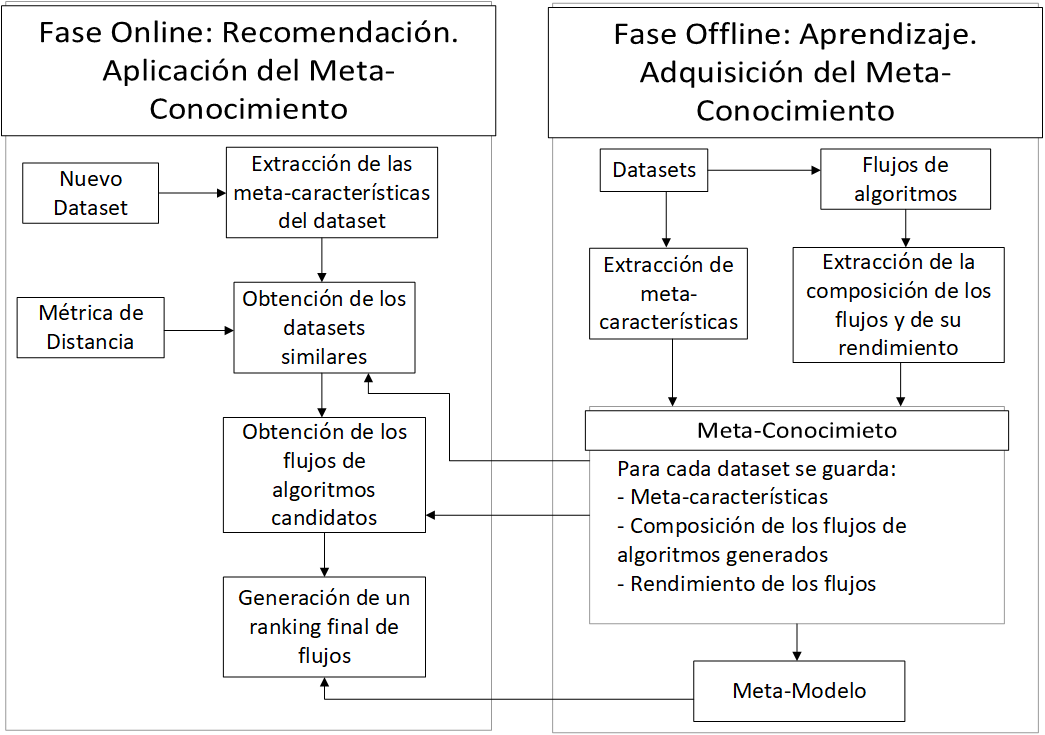
\includegraphics[scale=.5]{Figures/system.png}
	%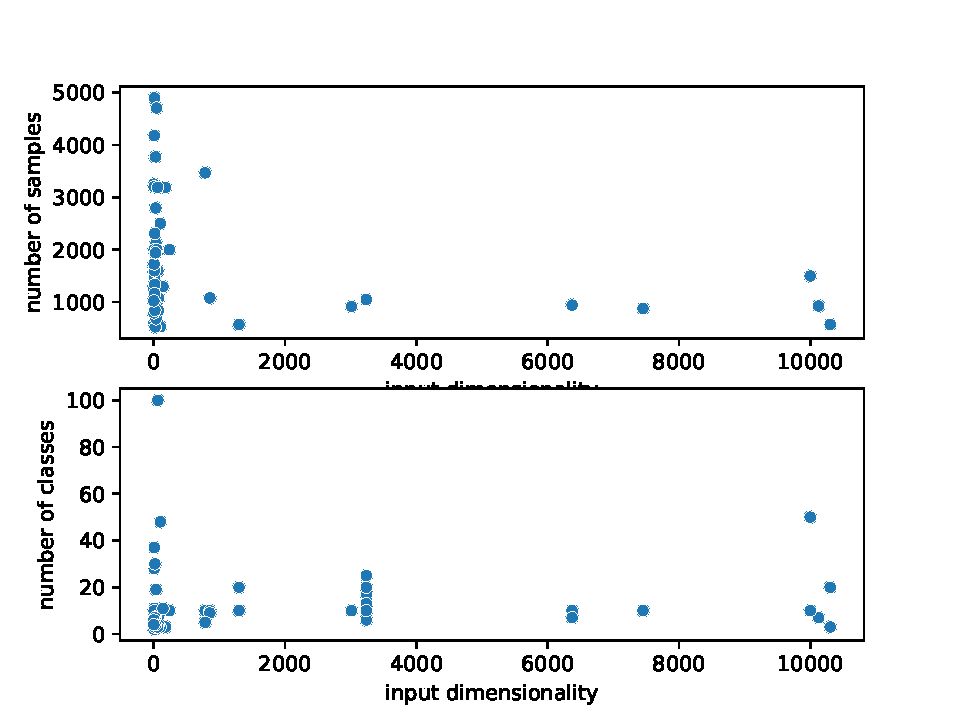
\includegraphics[scale=.60]{Figures/mtf scatterplot.pdf}
	\caption{Flujo de trabajo del enfoque de meta-learning propuesto.}
	\label{fig:system}
\end{figure}

% \begin{figure}[htb]
% 	\centering
% 	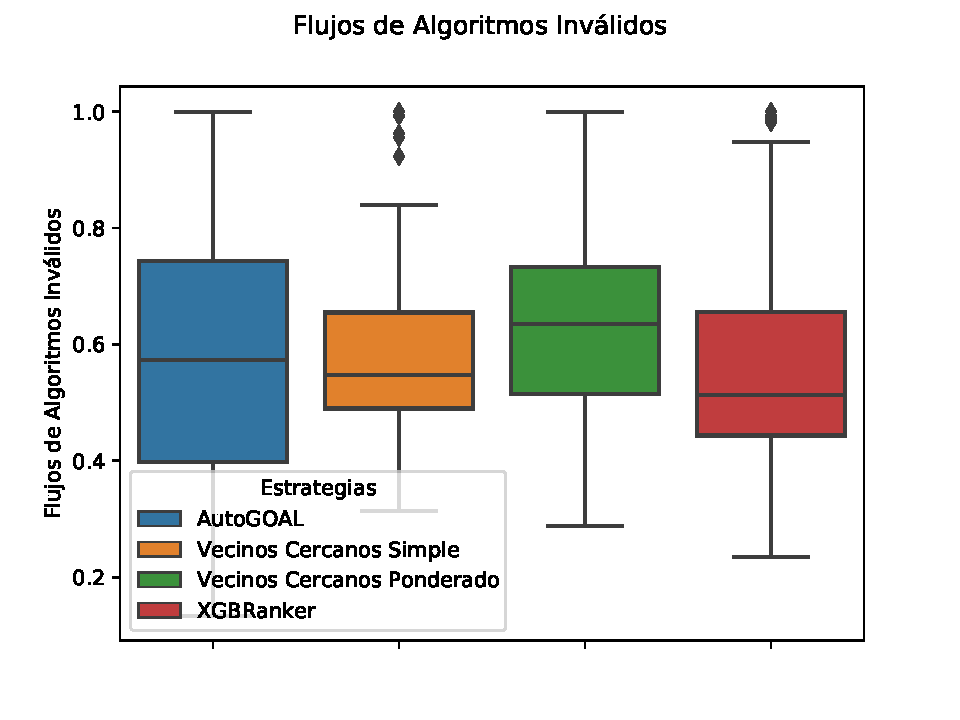
\includegraphics[scale=.8]{Figures/failed-pipelines.pdf}
% 	\caption{Proporción de flujos de algoritmos inválidos generados en cada uno datasets usando las diferentes estrategias.}
% 	\label{fig:failedpipelines}
% 	\end{figure}

\begin{figure}[htb]
	\centering
	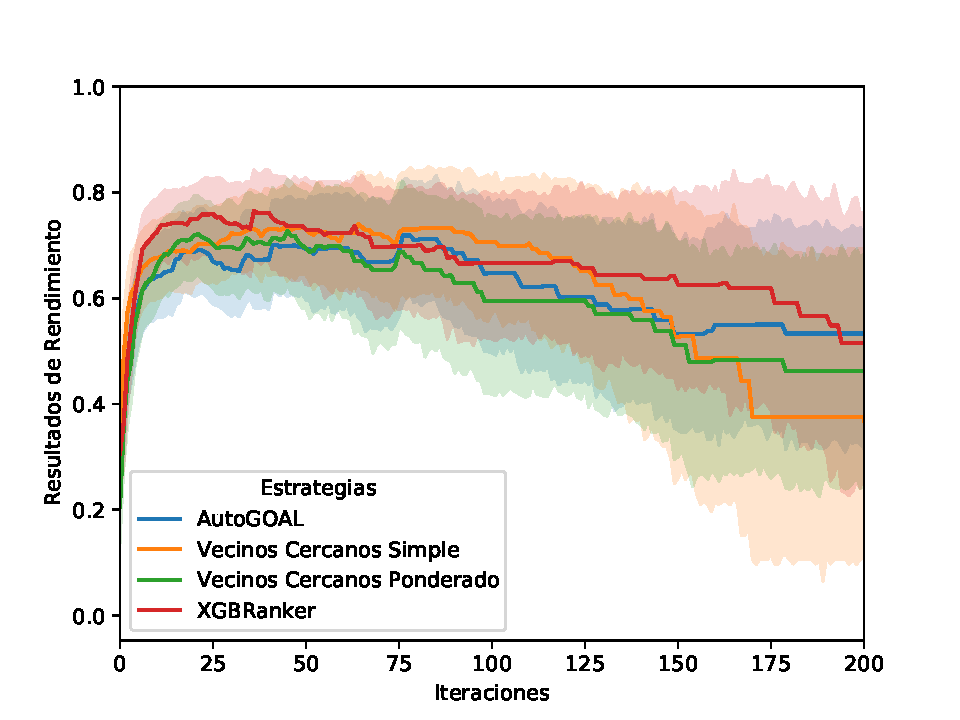
\includegraphics[scale=.8]{Figures/performance.pdf}
	\caption{Resultados de rendimiento obtenidos en los datasets de prueba en las primeras 200 iteraciones, se muestra la media y el intervalo de confianza del 95\%.}
	\label{fig:performance}
\end{figure}

\begin{figure}[htb]
	\centering
	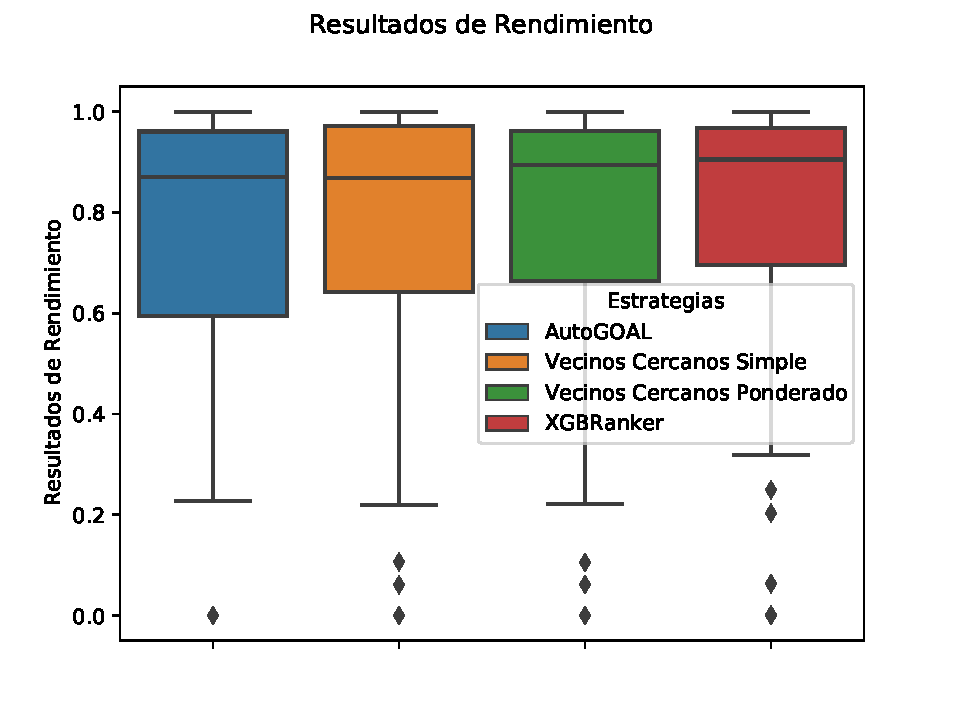
\includegraphics[scale=.8]{Figures/best-fn.pdf}
	\caption{Mejor resultado de rendimiento obtenido en la búsqueda de los flujos de algoritmos en cada uno de los datasets de prueba para las diferentes estrategias.}
	\label{fig:bestfn}
\end{figure}

\begin{figure}[htb]
	\centering
	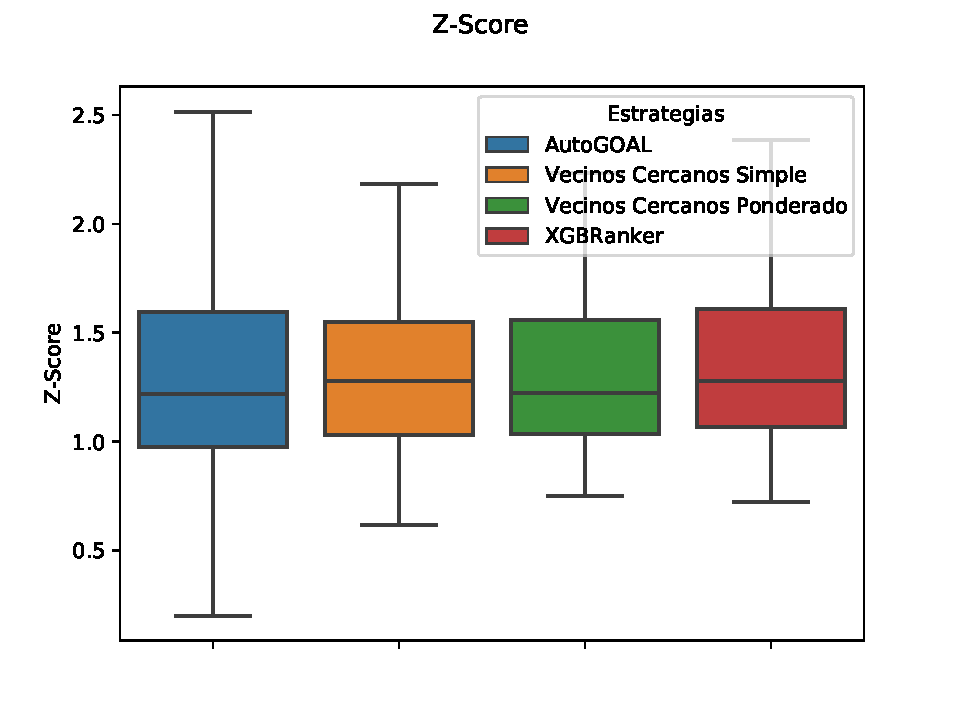
\includegraphics[scale=.8]{Figures/z-score.pdf}
	\caption{Puntuación Z obtenida en la búsqueda de los flujos de algoritmos en cada uno de los datasets de prueba para las diferentes estrategias.}
	\label{fig:zscore}
\end{figure}


%-------------------------------------------------------------------------
% DO NOT DELETE THIS.
% This is the end of the document.  Nothing else should go past this.
%-------------------------------------------------------------------------

\end{document}